\chapter{Introduction}
\label{chap: intro}
Remanufacturing has increasingly received attention because of its energy-saving, eco-friendly, and cost-efficient characteristics. Remanufactured products has been presented in automotive, aerospace, and industrial machinery industry. For example, in the automotive industry, Ford Motor has been recycled and remanufactured components such as engine, transmission, car body, etc., as a long-term tradition. In short, remanufacturing is a process of returning a used product to at least original performance specification from the customers’ perspective. To achieve this, ensuring the quality and reliability of incoming end-of-life (EoL) products by estimating the quantities of interest, e.g., remaining useful life (RUL) estimation and residual stress, becomes an essential step.

In recycled components, material fatigue damage is universally presented and it is one of the most influential factors that determines the RUL of a used product. Material fatigue has resulted in many catastrophic accidents in the history and has been studied for several decades; however, the fatigue damage level is hard to be monitored in real world environments due to the stochastic nature of fatigue behaviors and undetermined loading conditions \cite{fatigue-review-Santecchia2016}, which is a critical issue to be addressed.

To quantitatively study fatigue damage in materials, non-destructive evaluation (NDE) methods have been developed \cite{nde-review-WISNER2020}. NDE, also known as non-destructive testing (NDT), is a technique to evaluate material properties without causing damage to the testing parts. For instance, linear ultrasonic (LU) and nonlinear ultrasonic (NLU) testings send ultrasonic wave which propagates in a material and analyze the response signals to evaluate material degradation. Although there exists a variety of NDE techniques, each of these methods is only sensitive to a few specific fatigue conditions and is limited to detecting defects in certain length scales. Figure \ref{fig: lu nlu length scales} illustrates the detectable length scales of LU and NLU testings, where LU testing cannot detect defects much smaller than the probing wavelength (in e.g. stainless steels, typically on the order of 1mm). In contrast, NLU techniques measure nonlinear material parameters to detect defects which are orders of magnitude smaller than the probing wavelength.

\begin{figure}[tb]
    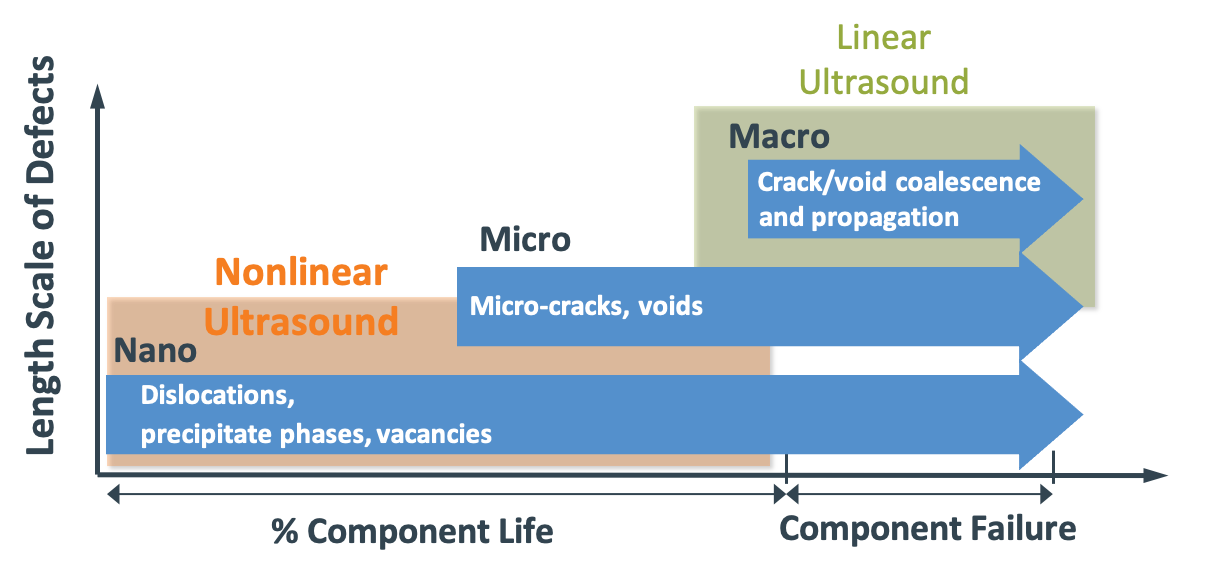
\includegraphics[width=\linewidth]{fig/lu_nlu_length_scales.png}
    \caption{Capability of defect detection for LU and NLU testings}
    \label{fig: lu nlu length scales}
\end{figure}